\documentclass[xcolor=dvipsnames,aspectratio=169,t]{beamer}
  % t means frames are vertically centered to the top
\usepackage{slides-header}
\title{Diagonalization}

\begin{document}
\maketitle

\begin{frame}{Diagonal Matrices}
  \medskip

  \alert{Diagonal matrices} are particularly nice to work with in many contexts, and can simplify calculations considerably.
  \bigskip
  
  Consider the matrix $D = \begin{bmatrix} 2 & 0 & 0 \\ 0 & 3 & 0 \\ 0 & 0 & 5 \end{bmatrix}$.
  \medskip
  
  \begin{itemize}
  \item We know $\det D = (2)(3)(5)=30$, and thus $D$ is invertible.
  \smallskip
  \item We know that $D$ has eigenvalues $\lambda = 2, 3, 5$.
  \smallskip
  \item We can easily raise $D$ to powers:
  \[ D^k = \underset{\text{$k$ times}}{\underbrace{D D \ldots D}} = \begin{bmatrix}2^k & 0 & 0 \\ 0 & 3^k & 0 \\ 0 & 0 & 5^k\end{bmatrix}. \]
  \end{itemize}
\end{frame}


\begin{frame}{Example}
  \medskip

  Recall this example where $\colorb{A}$ is \alert{similar} to the diagonal matrix $\alert{B}$.

  \[  \underbrace{\begin{bmatrix} -6 & -4 & -1 \\ -3 & -2 & -1 \\ 5 & 3 & 1 \end{bmatrix}}_{P^{-1}}
  \colorb{\underbrace{\begin{bmatrix} -13 & -8 & -4 \\ 12 & 7 & 4 \\ 24 & 16 & 7 \end{bmatrix}}_A }
  \underbrace{\begin{bmatrix} 1 & 1 & 2 \\ -2 & -1 & -3 \\ 1 & -2 & 0 \end{bmatrix}}_P  =
  \alert{\underbrace{\begin{bmatrix} -1 & 0 & 0 \\ 0 & 3 & 0 \\ 0 & 0 & -1 \end{bmatrix}}_B}. \]

  \begin{itemize}
  \item $A$ has \alert{eigenvalues} $\lambda = -1 ,3$ (with $\lambda = -1$ having multiplicity 2).
  \end{itemize}
  \smallskip
  
  \pause
  \begin{definition}
    An $n \times n$  matrix $A$ is said to be \alert{diagonalizable} if it is similar to a diagonal matrix $D$.
  \end{definition}

  \begin{itemize}
  \item Not all matrices are diagonalizable.
  \item How do we determine if a matrix is diagonalizable?
  
        If so, how can we find an invertible matrix $P$ such that $P^{-1}AP=D$?
  \end{itemize}
\end{frame}

\begin{frame}{Diagonalizable Matrices}
  \smallskip

  Suppose an $n \times n$ matrix $A$ is \alert{diagonalizable}.
  Then $A$ is is similar to a diagonal matrix $D$,
  \smallskip
  
  and there is an \blue{invertible matrix $P$} such that $P^{-1}AP=D$.
  Equivalently, $AP=PD$.
  \medskip
  
  {\small
  Let $P = \begin{bmatrix} \v_1 & \v_2 & \ldots & \v_n \end{bmatrix}
         = \begin{bmatrix}
             v_{11} & v_{12} & \ldots & v_{1n} \\
             v_{21} & v_{22} & \ldots & v_{2n} \\
             \vdots & \vdots & \ddots & \vdots \\
             v_{n1} & v_{n2} & \ldots & v_{nn}
           \end{bmatrix}$
  and $D = \begin{bmatrix} 
        d_1 & 0 & \ldots & 0 \\
        0 & d_2 & \ldots & 0 \\
        \vdots & \vdots & \ddots & \vdots \\
        0 & 0 & \ldots & d_n \end{bmatrix}$.
  }
  \medskip
  
  \pause
  We compute
    \begin{align*}
      AP &= \begin{bmatrix} A \v_1 & A \v_2 & \ldots & A \v_n \end{bmatrix}  \\
      PD &= \onslide<3->{\begin{bmatrix} d_1\v_1 & d_2 \v_2 & \ldots & d_n \v_n \end{bmatrix}}
    \end{align*}
  \vspace*{-.75em}
  
  \pause  % for onslide<3>
  \pause
  Since $A\v_i=d_i \v_i$, $d_i$ is an \alert{eigenvalue} of $A$ with corresponding \blue{eigenvector} $\v_i$.
  \bigskip
  
  \pause
  Since $P$ is \blue{invertible}, the columns of $P$ are \alert{linearly independent}.
  \smallskip
  
  \qquad Thus, the $\v_i$s are $n$ linearly independent \blue{eigenvectors} of $A$.
\end{frame}

\begin{frame}{Diagonalization Theorem}
  \medskip
  
  \begin{theorem}
  An $n \times n$ matrix $A$ is \alert{diagonalizable} if and only if 
  $A$ has \blue{$n$ linearly independent eigenvectors}.
  \bigskip
  
  If $A$ is diagonalizable, then $P^{-1}AP=D$ where:
  \begin{itemize}
  \item $P$ is an $n \times n$ matrix whose columns are the $n$ linearly independent eigenvectors.
  \item $D$ is an $n \times n$ diagonal matrix whose diagonal entries are the eigenvalues of $A$ that correspond, respectively, to the eigenvectors in $P$.
  \end{itemize}
\end{theorem}

  \[
    \scalebox{1.5}{$ P^{-1} A $}
    \underbrace{\begin{bmatrix} | & | &  & | \\ \v_1 & \v_2 & \ldots & \v_n \\ | & | & & | \end{bmatrix}}_P
    = 
      \underbrace{
      \begin{bmatrix} 
        \lambda_1 & 0 & \ldots & 0 \\
        0 & \lambda_2 & \ldots & 0 \\
        \vdots & \vdots & \ddots & \vdots \\
        0 & 0 & \ldots & \lambda_n \end{bmatrix}}_D
  \]
\end{frame}


\begin{frame}{A $2 \times 2$ Example}
  \bigskip

  Diagonalize if possible the matrix $A = \begin{bmatrix} 6 & -1 \\ 2 & 3 \end{bmatrix}$.
  \bigskip
  
  \pause
  We have
  \[ \begin{bmatrix} 6 & -1 \\ 2 & 3 \end{bmatrix} \begin{bmatrix} 1 \\ 1 \end{bmatrix} = \alert{5 \begin{bmatrix} 1 \\ 1 \end{bmatrix}} \quad \mbox{and} \quad  \begin{bmatrix} 6 & -1 \\ 2 & 3 \end{bmatrix} \begin{bmatrix} 1 \\ 2 \end{bmatrix} = \colorb{4 \begin{bmatrix} 1 \\ 2 \end{bmatrix}}. \]
  \medskip

  Thus \alert{$\lambda_1 = 5$ with eigenvector $\v_1 = \begin{bmatrix} 1 \\ 1 \end{bmatrix}$} and \colorb{$\lambda_2 = 4$ with eigenvector $\v_2 = \begin{bmatrix} 1 \\ 2 \end{bmatrix}$}.
  \bigskip
  
  \pause
  Since the eigenvectors $\alert{\v_1}$ and $\blue{\v_2}$ are linearly independent, we have
  \[ P^{-1}AP=
  \left( \begin{bmatrix} \alert{1} & \colorb{1} \\ \alert{1} & \colorb{2} \end{bmatrix} \right)^{-1} 
  \begin{bmatrix}6 & -1 \\ 2 & 3 \end{bmatrix} 
  \begin{bmatrix} \alert{1} & \colorb{1} \\ \alert{1} & \colorb{2} \end{bmatrix} 
  = 
  \begin{bmatrix} \alert{5} & 0 \\ 0 & \colorb{4} \end{bmatrix} 
  = D. \]
  
%   \pause
%   \[ \text{Check: }AP=\begin{bmatrix}6 & -1 \\ 2 & 3 \end{bmatrix}\begin{bmatrix} \alert{1} & \colorb{1} \\ \alert{1} & \colorb{2} \end{bmatrix} = \begin{bmatrix} \alert{5} & \colorb{4} \\ \alert{5} & \colorb{8} \end{bmatrix}
%   =  \begin{bmatrix} \alert{1} & \colorb{1} \\ \alert{1} & \colorb{2} \end{bmatrix} \begin{bmatrix} \alert{5} & 0 \\ 0 & \colorb{4} \end{bmatrix} =PD. \]
\end{frame}


\begin{frame}{Linear Independence of Eigenvectors}
  \begin{theorem}
  If $\v_1,\ldots,\v_p$ are eigenvectors corresponding to \colorr{distinct} eigenvalues $\lambda_1, \ldots, \lambda_p$ of an $n \times n$ matrix $A$, then the set $\left\{ \v_1, \ldots, \v_p \right\}$ is \colorr{linearly independent}.
  \end{theorem}
  %\vspace*{-1em}

  \pause
  {\small
  \blue{Proof.}
  Suppose $\left\{ \v_1, \ldots, \v_p \right\}$ is linearly dependent.
  Thus there are scalars $c_i$, not all zero, such that
  \vspace{-0.15in}
  \begin{equation}
  c_1 \v_1 + c_2 \v_2 + \ldots + c_p \v_p = \mathbf{0}.
  \end{equation}
  \vspace*{-0.3in}

  Among all such $c_i$s that are not all zero, choose the scalars such that the \colorb{fewest} $c_i$s are nonzero.
  Since the $v_i$s are eigenvectors and not the zero vector, at least two of the $c_i$s must be nonzero.  Assume that $c_j$ and $c_k$ are nonzero.

  \pause
  Multiplying both sides of equation (1) by $A$ gives
  \vspace{-0.15in}

  \begin{equation}
  A(c_1 \v_1 + \ldots +c_j \v_j + \ldots + c_p \v_p) = c_1 \lambda_1 \v_1 + \ldots +c_j \lambda_j \v_j + \ldots + c_p \lambda_p \v_p = \mathbf{0}.
  \end{equation}
  \vspace{-0.2in}

  \pause
  Multiplying both sides of equation (1) by $\lambda_j$ and subtracting from equation (2) gives
  \vspace{-0.15in}

  \begin{equation}
  c_1 (\lambda_1 - \lambda_j)\v_1 + c_2 (\lambda_2 - \lambda_j)\v_2 + \ldots + 0\v_j + \ldots + c_p (\lambda_p - \lambda_j)\v_p = \mathbf{0}.
  \end{equation}
  \vspace{-0.2in}

  \pause
  Note that $c_k (\lambda_k-\lambda_j)\ne 0$ since $\lambda_k\ne\lambda_j$.
  Thus, we have expressed $\mathbf{0}$ as a linear combination of $\v_1,\ldots,\v_p$ with not all scalars $0$ that has \colorb{fewer} nonzero scalars than what we assumed was the fewest. 
  \red{Contradiction!}
  \hfill\blue{\qed}
  }
\end{frame}


\begin{frame}{$3 \times 3$ Example 1}
  \smallskip

  If possible, diagonalize the matrix $A = \begin{bmatrix} 2 & 0 & 0 \\ 1 & 2 & 1 \\ -1 & 0 & 1 \end{bmatrix}$.
  \bigskip

  \bb
  \pause
  \ii \alert{Find the eigenvalues by solving the characteristic equation $\det (A - \lambda I) = \mathbf{0}$.}

  \[ \det (A - \lambda I) = \det \begin{bmatrix} 2 - \lambda &  0 & 0 \\ 1 & 2-\lambda & 1 \\ -1 & 0 & 1 - \lambda \end{bmatrix} = (2-\lambda)^2(1-\lambda) =0\]

  $A$ has eigenvalues $\lambda =2$ (with multiplicity 2) and $\lambda =1$.
  \bigskip

  \pause
  \ii \alert{If possible, find three linearly independent eigenvectors by solving $(A - \lambda I) \x = \mathbf{0}$.}
  \ee
\end{frame}

\begin{frame}
  \bb
  \setcounter{enumi}{1}
  \ii \alert{If possible, find three linearly independent eigenvectors by solving $(A - \lambda I) \x = \mathbf{0}$.}
  \ee

  \begin{columns}[T]

  \column{0.5\tw}

  {\small
  For \alert{$\lambda = 1$} we have: \ms

  $\begin{bmatrix} 2 - \alert{1} &  0 & 0 \\ 1 & 2-\alert{1} & 1 \\ -1 & 0 & 1 - \alert{1} \end{bmatrix} \x = \begin{bmatrix} \alert{1} & 0 & 0 \\ 1 & \alert{1} & 1 \\ -1 & 0 & \alert{0} \end{bmatrix} \x = \mathbf{0}$

  \bs

  if $\x = x_3 \alert{\begin{bmatrix} 0 \\ -1 \\ 1\end{bmatrix}}$. Thus the set  \alert{$\left\{ \begin{bmatrix} 0 \\ -1 \\ 1 \end{bmatrix} \right\}$} is a basis for the eigenspace corresponding to $\lambda =1$.
  }

  \column{0.5\tw}
  
  \pause
  {\small
  For \colorb{$\lambda = 2$} we have: \ms

  $\begin{bmatrix} 2 - \colorb{2} &  0 & 0 \\ 1 & 2-\colorb{2} & 1 \\ -1 & 0 & 1 - \colorb{2} \end{bmatrix} \x = \begin{bmatrix} \colorb{0} & 0 & 0 \\ 1 & \colorb{0} & 1 \\ -1 & 0 & \colorb{-1} \end{bmatrix} \x = \mathbf{0}$

  \bs

  if $\x = x_2 \colorb{\begin{bmatrix} 0 \\ 1 \\ 0\end{bmatrix}}+ x_3 \colorg{\begin{bmatrix} -1 \\ 0 \\ 1\end{bmatrix}}$. Thus $\left\{ \colorb{\begin{bmatrix} 0 \\ 1 \\ 0\end{bmatrix}},  \colorg{\begin{bmatrix} -1 \\ 0 \\ 1\end{bmatrix}} \right\}$ forms a basis for the eigenspace of $\lambda = 2$.}

  \end{columns}
  \medskip

  \pause
  \bb
  \addtocounter{enumi}{2}
  \ii \alert{Construct matrix $P$ from the vectors above.}

  \[ P = \begin{bmatrix} \alert{0} & \colorb{0} & \colorg{-1} \\ 
  \alert{-1} & \colorb{1} & \colorg{0} \\ 
  \alert{1} & \colorb{0} & \colorg{1} \end{bmatrix} \quad \mbox{and} \quad D = \begin{bmatrix} \alert{1} & 0 & 0 \\ 0 & \colorb{2} & 0 \\ 0 & 0 & \colorg{2} \end{bmatrix} .\]

  \ii \alert{Construct matrix $D$ from the corresponding eigenvalues.}
  \ee
\end{frame}

\begin{frame}{Checking our Work}
  \bb
  \ii Find the eigenvalues by solving the characteristic equation $\det (A - \lambda I) = \mathbf{0}$.
  \ii If possible, find $n$ linearly independent eigenvectors by solving $(A - \lambda I) \x = \mathbf{0}$.
  \ii Construct matrix $P$ from the vectors above.
  \ii Construct matrix $D$ from the corresponding eigenvalues.
  \ii \alert{Verify your results.}
  \ee

  \pause
  \[ P^{-1} A P = \left( \begin{bmatrix} 0 &0 & -1 \\ -1 & 1 & 0 \\ 1 & 0 & 1 \end{bmatrix}  \right)^{-1} 
  \alert{\begin{bmatrix} 2 & 0 & 0 \\ 1 & 2 & 1 \\ -1 & 0 & 1 \end{bmatrix}} 
  \begin{bmatrix} 0 &0 & -1 \\ -1 & 1 & 0 \\ 1 & 0 & 1 \end{bmatrix} = 
  \colorb{\begin{bmatrix} 1 & 0 & 0 \\ 0 & 2 & 0 \\ 0 & 0 & 2 \end{bmatrix}} = D.\]

  \pause
  Or you can check that
  {\scriptsize
  \[ AP = \alert{\begin{bmatrix} 2 & 0 & 0 \\ 1 & 2 & 1 \\ -1 & 0 & 1 \end{bmatrix}}
  \begin{bmatrix} 0 &0 & -1 \\ -1 & 1 & 0 \\ 1 & 0 & 1 \end{bmatrix} 
  = \colorg{\begin{bmatrix} 0 & 0 & -2 \\ -1 & 2 & 0 \\ 1 & 0 & 2 \end{bmatrix}}
  \quad  
  PD = \begin{bmatrix} 0 &0 & -1 \\ -1 & 1 & 0 \\ 1 & 0 & 1 \end{bmatrix} 
  \colorb{\begin{bmatrix} 1 & 0 & 0 \\ 0 & 2 & 0 \\ 0 & 0 & 2 \end{bmatrix}}
  = \colorg{\begin{bmatrix} 0 & 0 & -2 \\ -1 & 2 & 0 \\ 1 & 0 & 2 \end{bmatrix}} \]}
\end{frame}

\begin{frame}{Computing Powers of a Matrix}
  \medskip
  
  Compute $A^7$ for $A = \begin{bmatrix} 2 & 0 & 0 \\ 1 & 2 & 1 \\ -1 & 0 & 1 \end{bmatrix}$.
  \pause
  We previously showed that $A$ is \alert{diagonalizable}.
  
  Thus, there is an invertible matrix $P$ and a diagonal matrix $D$ such that $P^{-1}AP=D$.
  \medskip
  
  \pause
  Solving for $A$, we have that $\blue{A=PDP^{-1}}$.  Thus,
  \begin{align*}
  A^7 &=  \underset{7 \mbox{ times}}{\underbrace{(PDP^{-1}) (PDP^{-1}) \ldots (PDP^{-1})}} = P \underset{7 \mbox{ times}}{\underbrace{D(\alert{P^{-1}P})D(\alert{P^{-1}P}) \ldots  (\alert{P^{-1}P})D}}P^{-1} = P D^7 P^{-1} \\
  \onslide<4->{
  &=  
  \begin{bmatrix} 0 & 0 & -1 \\ -1 & 1 & 0 \\ 1 & 0 & 1 \end{bmatrix} 
  \begin{bmatrix} 1^7 & 0 & 0 \\ 0 & 2^7 & 0 \\ 0 & 0 & 2^7 \end{bmatrix} 
  \begin{bmatrix} 0 & 0 & -1 \\ -1 & 1 & 0 \\ 1 & 0 & 1 \end{bmatrix}^{-1} 
  = \begin{bmatrix} 128 & 0 & 0 \\ 127 & 128 & 127 \\ -127 & 0 & 1 \end{bmatrix}
  }
  \end{align*}
  \smallskip
  
  \pause
  \pause
  
  In general, $\alert{A^k} = (PDP^{-1})^k = P \alert{D^k} P^{-1}$ for a positive integer $k$.
\end{frame}


\begin{frame}{$3 \times 3$ Example 2}
  \medskip

  If possible, diagonalize the matrix $A = \begin{bmatrix} 2 & 4 & 6 \\ 0 & 2 & 2 \\ 0 & 0 & 4 \end{bmatrix}$.
  \pause Since $A$ is \blue{triangular}, its eigenvals are $2,4$.
  
  \vspace{-0.05in}

  \pause
  For \alert{$\lambda =4$} we have

  \[ (A-4I)\x = \begin{bmatrix} -2 & 4 & 6 \\ 0 & - 2 & 2 \\ 0 & 0 & 0 \end{bmatrix} \x = \mathbf{0} \mbox{ when } \x =x_3 \begin{bmatrix} 5 \\ 1 \\ 1 \end{bmatrix} 
  \mbox{, thus a basis is } \left\{ \begin{bmatrix} 5 \\ 1 \\ 1 \end{bmatrix} \right\}.\]
  
  \vspace{-0.05in}

  \pause
  For \blue{$\lambda =2$} we have

  \[ (A-2I)\x = \begin{bmatrix} 0 & 4 & 6 \\ 0 & 0 & 2 \\ 0 & 0 & 2 \end{bmatrix} \x = \mathbf{0} \mbox{ when } \x =x_1 \begin{bmatrix} 1 \\ 0 \\ 0 \end{bmatrix} \mbox{, thus a basis is } \left\{ \begin{bmatrix} 1 \\ 0 \\ 0 \end{bmatrix} \right\} .\]
  \smallskip

  \pause
  Since we do \alert{\textbf{NOT}} have three linearly independent eigenvectors, $A$ is \alert{\textbf{NOT diagonalizable.}}
\end{frame}


\begin{frame}{$3 \times 3$ Example 3}
  \medskip

  Determine whether or not $A = \begin{bmatrix} 3 & 2 & 1 \\ 0 & 6 & 2 \\  0 & 0 & 2 \end{bmatrix}$ is diagonalizable.
  \bigskip

  \pause
  \bi
  \ii Notice matrix $A$ is \blue{upper triangular}, so $A$ has eigenvalues $\lambda = 3, 6, 2$.\ms
  \pause
  \ii If $\v_1$, $\v_2$, and $\v_3$ are eigenvectors corresponding to \alert{distinct} eigenvalues $\lambda_1$, $\lambda_2$, and $\lambda_3$, then we proved that the set of eigenvectors $\left\{ \v_1, \v_2, \v_3 \right\}$ is \blue{linearly independent}. \ms
  \pause
  \ii Since $A$ has \blue{three linearly independent eigenvectors}, it must be diagonalizable.
  \ei
  \bigskip

  \pause
  \begin{theorem}
  An $n \times n$ matrix with \alert{$n$ distinct eigenvalues} is diagonalizable.
  \end{theorem}
\end{frame}


\begin{frame}{Matrices with Eigenvalues of Higher Multiplicity}
  \begin{theorem}
  Let $A$ be an $n \times n$ matrix whose distinct eigenvalues are $\lambda_1, \ldots , \lambda_p$.
  \bb[(a)]
  \ii For $1 \leq k \leq p$, the \blue{dimension of the eigenspace} for $\lambda_k$ (called the \emph{geometric multiplicity}) is at most the algebraic multiplicity of the eigenvalue $\lambda_k$.
  \medskip
  \pause
  \ii The matrix $A$ is diagonalizable if and only if the sum of the dimensions of the eigenspaces equals $n$.  This happens if and only if:
    \bb[(i)]
    \ii The characteristic polynomial factors completely into linear factors, and
    \ii The dimension of the eigenspace for each $\lambda_k$ \blue{equals} the multiplicity of $\lambda_k$.
    \ee
  \medskip
  \pause
  \ii If $A$ is diagonalizable and $\B_k$ is a basis for the eigenspace corresponding to eigenvalue $\lambda_k$, then all the vectors in the sets $\B_1, \ldots, \B_p$ form an \blue{eigenvector basis} for $\R^n$.
  \ee
\end{theorem}

\end{frame}

\begin{frame}{Reviewing Previous Examples}
  \medskip

\begin{columns}[T]

\column{0.33\tw}

The matrix $A = \begin{bmatrix} 2 & 0 & 0 \\ 1 & 2 & 1 \\ -1 & 0 & 1 \end{bmatrix}$ has eigenvalues: 

\bi 
\ii $\lambda =2$ with eigenspace dimension equal to 2, and
\ii $\lambda =1$ with eigenspace dimension equal to 1.
\ii $2 + 1 = 3$, so $A$ is diagonalizable.
\ei

\column{0.33\tw}

\pause
\alert{The matrix $A = \begin{bmatrix} 2 & 4 & 6 \\ 0 & 2 & 2 \\ 0 & 0 & 4 \end{bmatrix}$ has eigenvalues: 

\bi 
\ii $\lambda =2$ with eigenspace dimension equal to 1, and
\ii $\lambda =4$ with eigenspace dimension equal to 1.
\ii $1 + 1 = 2$, so $A$ is NOT diagonalizable.
\ei
}

\column{0.33\tw}

\pause
\colorb{The matrix  $A = \begin{bmatrix} 3 & 2 & 1 \\ 0 & 6 & 2 \\  0 & 0 & 2 \end{bmatrix}$ has eigenvalues:} 

\bi 
\ii \colorb{$\lambda =3, 6, 2$.}
\ii \colorb{Since $A$ has three distinct eigenvalues, it is diagonalizable.}
\ei

\end{columns}
\end{frame}


\begin{frame}{Interpretation of Similarity}
  \bigskip
  
  Suppose that $A$ is an $n\times n$ \red{diagonalizable} matrix: $A=PDP^{-1}$.
  \smallskip
  
  The columns of $P$ are bases for the eigenspaces of $A$, and together form a \colorr{basis $\B$}  for $\R^n$.
  \medskip
  
  Consider the linear transform $T\colon\R^n\to\R^n$ given by $T(\x)=A\x = PDP^{-1}\x$.
  \bigskip
  
  \pause
  $P$ is the \blue{change of basis} matrix from $\B$ to the standard basis.
  \smallskip
  
  $P^{-1}$ is the change of basis matrix from the standard basis to $\B$.
  \bigskip
  
  So to perform $T$ on a vector $x$ with respect to the standard basis, we can 
  \begin{enumerate}
    \item change to the basis $\B$ by multiplying by $P^{-1}$,
    \item then scale each coordinate by multiplying by $D$,
    \item then change back to the standard basis by multiplying by $P$.
  \end{enumerate}
\end{frame}


\begin{frame}{Example}
  \bigskip
  
  Consider the linear transform $T\colon\R^2\to\R^2$ given by 
  $T(\x)=A\x=\begin{bmatrix} 1.5 & 0.5 \\ 1 & 1 \end{bmatrix}\x$.
  \bigskip
  
  \begin{columns}[T]
  \column{.55\textwidth}
  \begin{align*}
    A&=PDP^{-1} \\
    &=
    \begin{bmatrix} 1 & -1\\1 & 2\end{bmatrix}
    \begin{bmatrix}2 & 0\\0 & 0.5\end{bmatrix}
    \left( \begin{bmatrix} 1 & -1\\1 & 2\end{bmatrix} \right)^{-1}.
  \end{align*}
  \smallskip
  
  {\small
  Desmos: \url{https://www.desmos.com/calculator/n7l5cf9xjo}
  }

  \column{.4\textwidth}
  \pause
  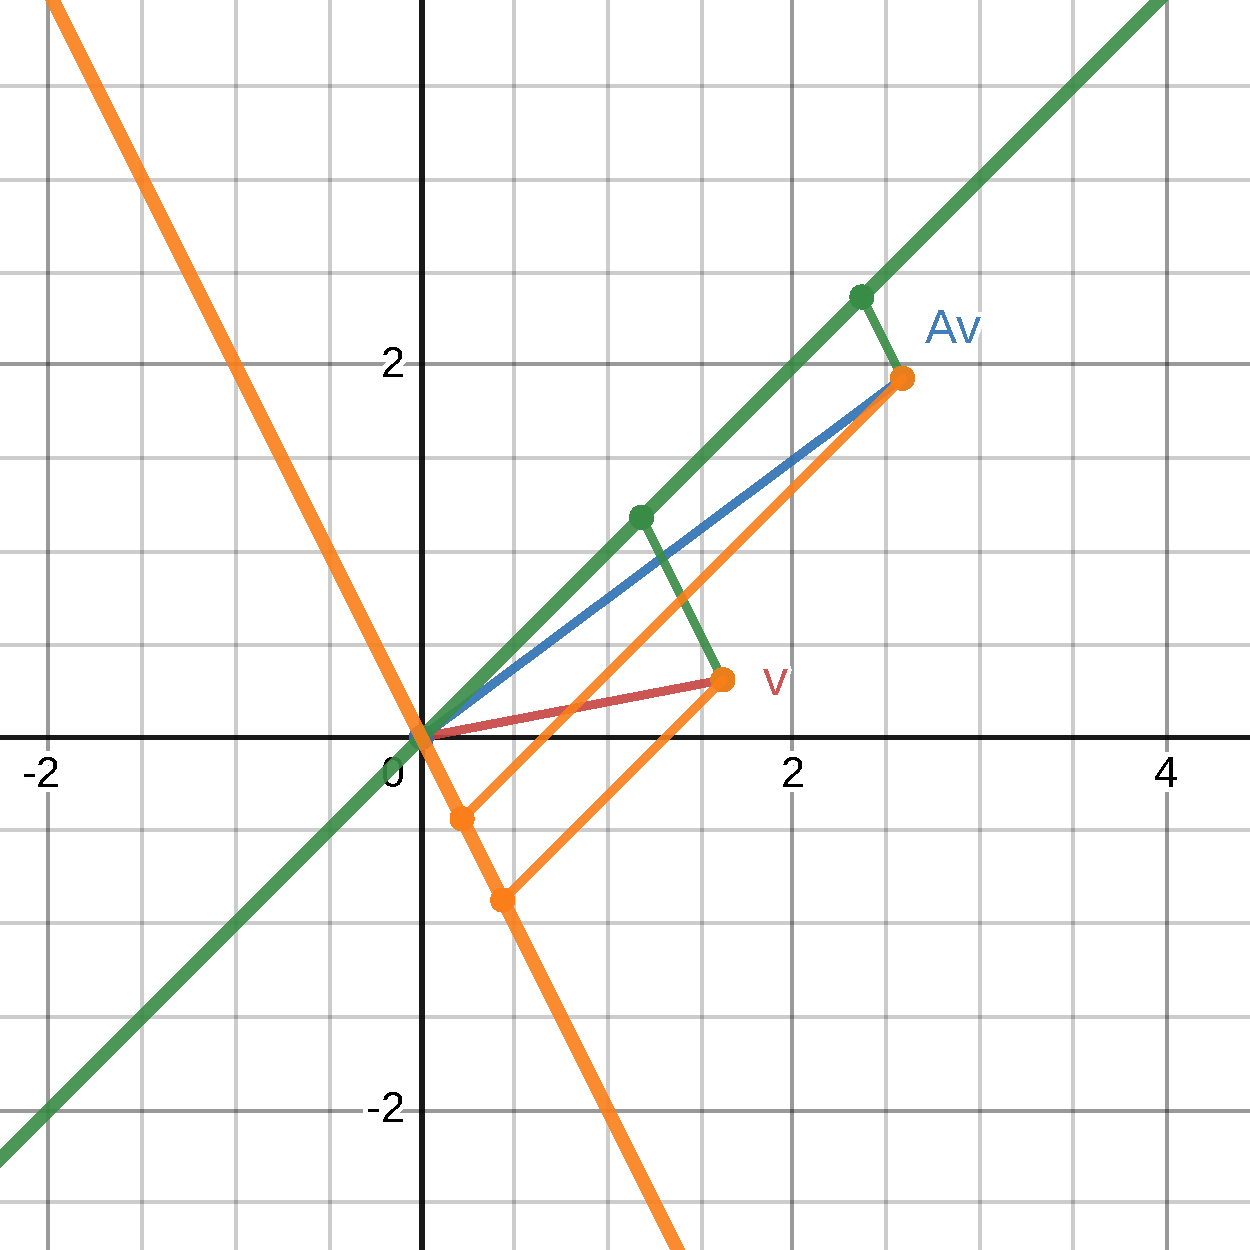
\includegraphics[scale=.25]{images/desmos-eigenvalues_linear_transformation.pdf}
  \end{columns}
\end{frame}

\end{document}

